\documentclass{LSkill} 

\usepackage{hyperref} 
\usepackage{graphicx} 
\usepackage{amsmath}   
\usepackage{amssymb}   

% Title ,Subtitle, author and date
\title{Project 2-1 \\ \large{---}} 
\author{
    Cem Andrew Gültekin, Antonie Bostan, Vincent Helms, Mikle Kuzin, \\ 
    Kamil Lipiński, Calin Suconicov, Greg Vadász
}
\date{\today}

\begin{document}


\maketitle
\tableofcontents

% Abstract
\begin{abstract}
Multi agent training is a specific branch of reinforcement learning in which a group of agents are trained to achieve a task together. What this means, is that the performance of agents are measured by group, and not by personal performance. Their policies are also collective. This style of reinforcement learning allows researchers to implement studies on team-based games, such as football, which is what this study will be investigating. The study will look to optimize the learning of agents with realistic sensors to score goals in a 2 versus 2 format, based on the POCA algorithm. 
\end{abstract}

% Introduction
\section{Introduction}
The primary objective of this study is to identify the most optimal configuration for training a set of agents to play football using POCA using the unity platform. The POCA algorithm was chosen due to its capability to efficiently support multi-agent learning. Thus, the primary research question for this study is “How can the training of agent clusters using POCA be optimized in order to teach them to play football in unity?”.

However, this question is quite broad as there is a lot to cover under the umbrella of optimising a reinforcement learning algorithm for training agents for a specific task. Therefore, these researchers have decided to break down this broad primary research question into three sub-questions, each exploring a different aspect of this optimization. The three questions are; What is the most suitable set of values for the configuration file of a POCA training algorithm for this task? What is the optimal combination of realistic sensors for performance for this task? Does training in the unity editor alter the performance of the agents when compared to training in a pre-compiled file? 

When researching the topic of Multi Agent Reinforcement Learning (MARL), we found that the majority of studies were fairly broad, and few focused on optimising MARL for a very specific, niche task such as playing football. Studies such as L. Bus¸oniu et al. and many more carry out much larger analyses on MARL as a whole, without diving into the specifics of POCA, especially not for a single task. In the field of MARL for football, we were able to find one single study which utilised PPO for a full 11 versus 11 football match simulation (Smit et al). However, although PPO has been described as an effective MARL algorithm, it was not the algorithm’s original purpose (Yu et al). Thus, we believe that by attempting to reconfigure the football game to be a 2 versus 2 scenario, as well as using the POCA algorithm instead of the PPO algorithm, we will be contributing something new to the MARL field of study.


In this study, we aim to discover if we can improve the football playing abilities of 4 agents in a 2v2 closed pitch scenario. We aim to do this using a POCA reinforcement learning algorithm, giving the agents both positive and negative rewards for certain actions. Ideally, as the agents experience playing they develop strategies to maximize the amount of positive rewards that they receive, using the POCA algorithm. We could not find any studies related to the specific task of training agents to play football using a POCA algorithm, thus we believe that our paper will be a novelty in this sense. As this study will be breaking down and exploring a very niche facet of multi-agent reinforcement learning, we believe that this study will be contributing to the current academic state of the art of reinforcement learning. 

\section{Methods}
In order to determine the most effective configuration of our training, we decided to use an Elo rating system. Out of all possible metrics we chose Elo rating as it is a very objective look at the performance of agents, which is the ultimate goal of this study. 
How Elo rating works in this context is the following. We have two opposing teams with specific policies. One team has the latest policy, whilst the other team has a previous policy, which gets switched up every so often. The teams play against each other, until one team wins. In this case the win is determined by who can score a goal first. The Elo of both teams is then adjusted after every round, based on who won as well as the previous Elo rating of both teams. Comparing the Elo ratings when adjusting is important, because the perceived improvement of either team is dependent on how good the other team supposedly is. Therefore having a set change to Elo rating doesn’t work.
Out of the two teams, one is the team that is currently  being trained, and the other is the “supporting” team. Both teams have their own respective Elo rankings, which start off at 1200. The Elo of each team develops as they play games against each other. The Elo score is calculated after every round, based on the Elo scores of both teams before the round started based on the following formula: 

\begin{figure}[htbp]
    \centering
    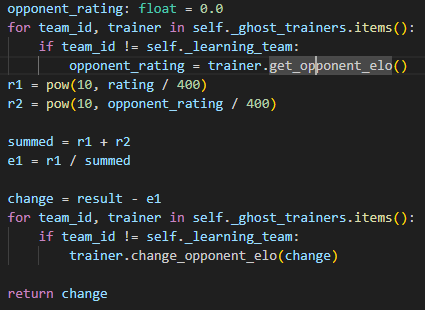
\includegraphics[width=0.5\textwidth]{figure 1.png} 
    \caption{Formula Of Elo Calculation}
    \label{fig:Formula Of Elo Calculation}
\end{figure}
By comparing the teams over multiple iterations, we can see how the reinforcement learning policies develop, and whether they are improving when compared to previous versions. Thus, Elo rating is an effective and reliable way to measure the improvement of the reinforcement learning policies overtime that the training algorithm develops. 
We used the Elo measurements provided by our POCA algorithm as a way of measuring the progress of the agent groups. More Elo progression meant better policy development, thus more optimal learning. 



\subsection{Method for Learning Algorithm Parameters Testing}
To find the optimal parameters of a learning algorithm like POCA we make runs with one parameter changed each time. Before the run we change the parameter we would like to make tests on from the configuration file (SoccerTwos.yaml in this case). For our tests we tested each parameter 3 times with the default value, a higher value and a lower value. For example hidden units:  256,  512,  1024. With 512 being the default. For each comparison the number of steps were kept the same.

\subsection{Methods for in-editor vs pre-compiled training comparison}
In this experiment, we use previously found optimal parameters.

In order to run the in-editor training, we have to run a command in the terminal: 
\texttt{mlagents-learn (path to)SoccerTwosBest.yaml --run-id=run\_1\_in\_editor}. We have to specify the path to the yaml file responsible for the training (\texttt{SoccerTwosBest.yaml} in this case). We also need to give a name to the run\_id. We call one training \texttt{run\_1\_in\_editor} and the second one \texttt{run\_2\_in\_editor}. When we enter the command, we run the scene in the Unity Editor.

In order to run the pre-compiled training, we first compile the Unity scene that we want to train the ML agents on into an executable file. To do this, we open the Unity Editor, go to \texttt{File -> Build Settings… -> Add open scenes}, and add the correct scene - \texttt{SoccerTwos} in this case. Then we click Build. We have to choose a folder in which the executable scene will be stored. 
We created a new folder called \texttt{Build} and chose this folder. 

Next, the scene is compiled. When it is ready, we have to run a command in the terminal: \texttt{mlagents-learn (path to) \textbackslash SoccerTwosBest.yaml --env (path to) \textbackslash UnityEnvironment.exe --run-id run\_1\_pre\_compiled --no-graphics}. We have to specify the path to the yaml file responsible for the training (\texttt{SoccerTwosBest.yaml} in this case) and the path to the executable environment (\texttt{UnityEnvironment.exe} in our case). We also need to give a name to the run\_id. We call one training \texttt{run\_1\_pre\_compiled} and the second one 
\texttt{run\_2\_pre\_compiled}. We also used \texttt{--no-graphics}, so the graphics 
of the scene are not generated, saving some computational power.

\subsection{Method for Sensor Testing:}
In order to compare the performances of different sensors, an in-editor training setup with the hyperparameters previously acquired were used. Three different sensor configurations were compared; Ray perception only, sound sensor only, ray perception and sound sensor combined. The ray perception sensor was a series of rays connected to the agent in a 120 FOV, in order to simulate realistic vision for the agent. The sound sensor was set up as an audio listener within the game with a set radius. The ball was set to trigger a noise when it came into contact with an agent or a ball. The agents were then notified of this noise. Logically, when combined, the sensors would constitute the two most important senses of a football player. Hearing and sound. Thus this configuration would produce the best results. In order to compare how individual configurations of the sensors perform we ran a training set using the POCA training algorithm for 2 million steps for each algorithm. This way, all configurations could be compared in an objective manner side by side. 
Elo rating is a viable way to compare how sensor types perform because certain sensor types should see faster progression in Elo rating than others. For example, we expected the sound sensors to have lower levels of Elo development, as it would take longer for agents to figure out what was happening in the beginning, thus leading to more ties. Ties should not influence Elo too much. 

%EXPERIMTENS    
\section{Experiments}

We have employed Bayesian optimization, facilitated by the Optuna framework, to automatically tune the hyperparameters of the PPO algorithm. The core objective was to maximize the Elo rating achieved by trained agents, serving as a proxy for overall performance within the game. The implementation leveraged a modular design, comprising several key stages:

\subsection{Configuration Generation and Dynamic Parameterization}

A base configuration file, specified in YAML format, defined the core structure and parameters of the PPO agent. A \texttt{create\_temp\_trainer\_config} function dynamically modified this configuration based on hyperparameters proposed by Optuna. Specifically, the following hyperparameters were included in the search space:

\begin{itemize}
    \item \textbf{learning\_rate}: A continuous parameter controlling the step size of the optimizer, sampled logarithmically between \texttt{1e-5} and \texttt{1e-3}.
    \item \textbf{batch\_size}: A categorical parameter defining the size of mini-batches used in the optimization process, selected from options \{\texttt{512}, \texttt{1024}, \texttt{2048}\}.
    \item \textbf{buffer\_size}: A categorical parameter that governs the size of the experience replay buffer, with options \{\texttt{2048}, \texttt{4096}, \texttt{8192}\}.
    \item \textbf{beta}: A continuous parameter defining the strength of the entropy bonus, sampled between \texttt{0.0001} and \texttt{0.01}.
    \item \textbf{num\_layers}: An integer parameter specifying the number of layers in the neural network, with options \{\texttt{1}, \texttt{2}, \texttt{3}\}.
    \item \textbf{hidden\_units}: A categorical parameter defining the number of hidden units in each layer, with options \{\texttt{128}, \texttt{256}, \texttt{512}\}.
\end{itemize}

These hyperparameter suggestions were integrated into a modified configuration file, which was stored temporarily for use in each trial. This approach allowed for iterative exploration of the hyperparameter space, with each trial using unique settings.
\subsection{Training and Performance Evaluation}

The \texttt{run\_training\_and\_get\_score} function executed the training process using the \texttt{mlagents-learn} command-line tool. The generated temporary configuration was provided as an argument, along with the path to the simulation environment. To manage resources and monitor the training, the following steps were taken.

The training progress was logged to a console output file, enabling retrospective analysis of the training process as well as providing key performance metrics, as the version of the ML-Agents we were using didn’t have proper support to parse the TensorBoard files in runtime.

The training procedure was set for a predefined duration of 500,000 steps in each trial. The \texttt{parse\_from\_console} function then analyzed the console output log, extracting the final Elo rating achieved by the trained agents. This metric served as the objective function to be maximized by the Bayesian optimization process.
\subsection{ Bayesian Optimization and Iterative Search:}
The Optuna framework's Bayesian optimization algorithm, which uses a Gaussian process as a surrogate model of the objective function, was applied to iteratively explore the hyperparameter search space.

A study was established using the SQLite storage backend to store the history of trials, allowing for continuation of optimization if necessary. The direction of optimization was set to "maximize", in order to achieve the highest ELO value as the desired outcome.

The objective function consolidated the configuration generation, training execution, and performance evaluation phases. After each trial was finished, the temporary configuration file was deleted to maintain a clean working directory.

The best result was saved and outputted to the console including the ELO and the hyperparameters that produced that result.

The script was run until for 10 consecutive runs no improvement could be noted and resulted in the following hyperparameters:


\begin{verbatim}
    batch_size: 512
    buffer_size: 4096
    beta: 0.0020460882794934116
    hidden_units: 512
    num_layers: 1
\end{verbatim}

\subsection{Finding The Optimal Learning Rate}
Our second experiment is making 3 runs with different learning rates in the SoccerTwos environment. The goal is to find the optimal learning rate by examining the models performance, convergence speed, CPU/GPU usage and framerate of the simulations. The 3 learning rates are 0.0001, 0.0003 and 0.0009. The runs will be examined until 3.5 million steps.

\subsection{Finding The Optimal Hidden Unit Number}
Our third experiment is making 3 runs with different hidden unit numbers in the SoccerTwos environment. The goal is to find the optimal hidden unit number by examining the models performance, convergence speed, CPU/GPU usage and framerate of the simulations. The 3 hidden unit numbers are 256, 512 and 1024.
 
\section{Results}
\subsection{Finding The Optimal Learning Rate}
As shown in Figure~\ref{fig:Cumulative Reward For Learning Rates}, the learning rates from grey to orange are 0.0009, 0.0003 and 0.0001. It takes 320 thousand steps for 0.0009 to get to max cumulative reward. 510 thousand steps for 0.0003 and 640 thousand for 0.0001.

So the learning rate of 0.0009 was able to reach the maximum cumulative reward significantly faster than the rest. The 0.0001 learning rate took the longest and 0.003 was somewhere between. And all of the learning rates converged before 650 thousand steps.


\begin{figure}[htbp]
    \centering
    \includegraphics[width=0.5\textwidth]{figure 2.png} 
    \caption{Cumulative Reward For Learning Rates}
    \label{fig:Cumulative Reward For Learning Rates}
\end{figure}

If we look at Figure~\ref{fig:ELO For Learning Rates} which shows us how the ELO changes throughout the run we can see 0.0009 starts well compared to the others. After 500 thousand steps each of the learning rates increase their elo steadily almost at the same rate. So at the end at 3.5 million steps the results are the same as the beginning.

\begin{figure}[htbp]
    \centering
    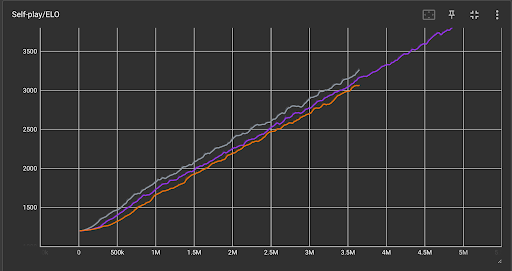
\includegraphics[width=0.5\textwidth]{figure 3.png} 
    \caption{ELO For Learning Rates}
    \label{fig:ELO For Learning Rates}
\end{figure}

Now if we look at Figure~\ref{fig:Baseline Loss For Learning Rates} for the baseline loss we can see 0.0009 is the first to converge to the final range. After that 0.0003 is the second and 0.0001 is the last.

\begin{figure}[htbp]
    \centering
    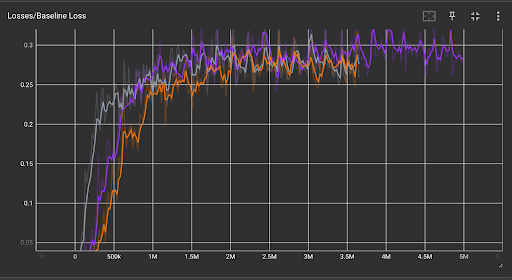
\includegraphics[width=0.5\textwidth]{figure 4.png} 
    \caption{Baseline Loss For Learning Rates}
    \label{fig:Baseline Loss For Learning Rates}
\end{figure}
\vspace{1cm}

There wasn’t much of a difference in the time it took for 3.65 million steps. 

\begin{verbatim}
	0.0009 learning rate took 6.872 hr
	0.0003 learning rate took 6.203 hr
	0.0001 learning rate took 6.999 hr
\end{verbatim}

	Frame Count in 3.65 million steps:

\begin{verbatim}
	0.0001 learning rate 548862 frames
	0.0003 learning rate 547517 frames
	0.0009 learning rate 547493 frames
\end{verbatim}

If we look at the CPU Usage on scripts and rendering both 0.0001 and 0.0009 learning rates have a lot of spikes in ms throughout the run. They jump to 66ms(15FPS) from 33ms(30FPS). While the run with 0.0003 mostly stays around 33ms(30FPS).
(APPENDIX A)
\vspace{0.5cm}

At Figure~\ref{fig:CPU Performance For Learning Rates} we have the CPU processing times from the main thread at the last frame of each run. The total CPU frame time is lowest at 0.0003 learning rate with 627.10ms making it the most efficient. The longest total CPU Frame time is at 0.0001 learning rate with 935.45ms. But it has the lowest number in the other 3 categories with most of its time on Render Loop.

\begin{figure}[htbp]
    \centering
    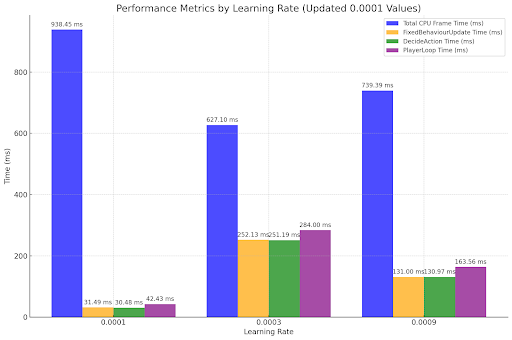
\includegraphics[width=0.5\textwidth]{figure 5.png} 
    \caption{CPU Performance For Learning Rates}
    \label{fig:CPU Performance For Learning Rates}
\end{figure}
\vspace{0.5cm}
Finally if we look at the memory usage of all at Figure~\ref{fig:Total Commited Memory By Learning Rates}. We can see that there is no significant relation between the learning rate and total committed memory.

\begin{figure}[htbp]
    \centering
    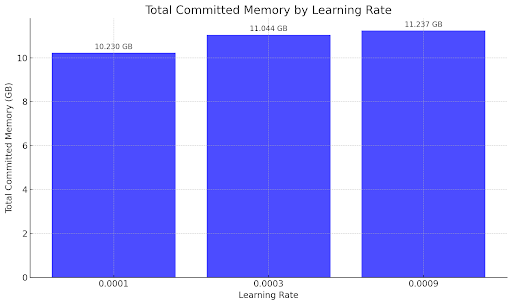
\includegraphics[width=0.5\textwidth]{figure 6.png} 
    \caption{Total Commited Memory By Learning Rates}
    \label{fig:Total Commited Memory By Learning Rates}
\end{figure}

\subsection{Finding The Optimal Hidden Unit Number}
To start with the cumulative reward if we look at Figure~\ref{fig:Cumulative Reward For Hidden Units} from orange to purple the hidden unit numbers go as 1024, 256 and 512. The run with 1024 hidden units is the first to converge at 320 thousand steps. After that the run with 256 hidden units converges at 510 thousand steps and the run with 512 units converges last at 520 thousand steps.

As we can see the run with 1024 units converges first but it suffers a big drop around 500 thousand steps. After that others converge before it can get back to maximum reward. But at the end all of them manage to converge around 500 thousand steps.

\begin{figure}[htbp]
    \centering
    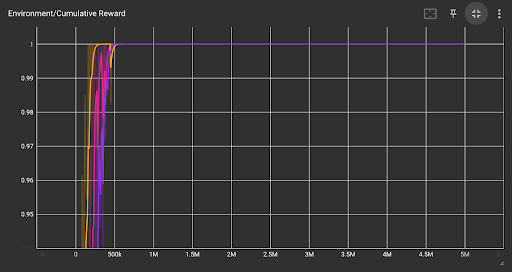
\includegraphics[width=0.5\textwidth]{figure 7.png} 
    \caption{Cumulative Reward For Hidden Units}
    \label{fig:Cumulative Reward For Hidden Units}
\end{figure}

Now if we have a look at ELO of the runs at Figure~\ref{fig:ELO For Hidden Units} the run with 1024 units starts off faster than the others and leads towards the end. After the start all of them continue to rise steadily at the same pace. So at the end they have very similar ELO’s. At 3.65 the highest elo is at 1024 units and the lowest is 512.

\begin{figure}[htbp]
    \centering
    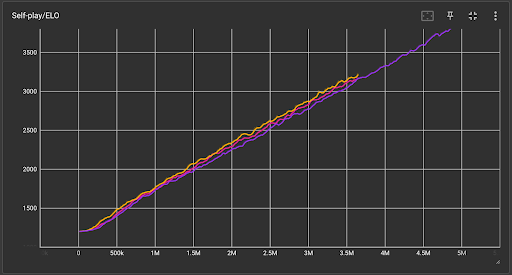
\includegraphics[width=0.5\textwidth]{figure 8.png} 
    \caption{ELO For Hidden Units}
    \label{fig:ELO For Hidden Units}
\end{figure}

When we look at Figure~\ref{fig:Baseline Loss For Hidden Units} for Baseline Loss the first to converge to the final range is 1024 units and the last is 256 units.

\vspace{0.5cm}
\begin{figure}[htbp]
    \centering
    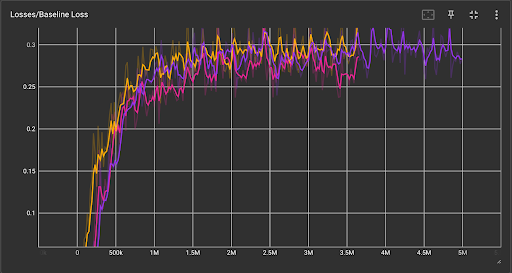
\includegraphics[width=0.5\textwidth]{figure 9.png} 
    \caption{Baseline Loss For Hidden Units}
    \label{fig:Baseline Loss For Hidden Units}
\end{figure}

Time difference for 3.65 million steps

\begin{verbatim}
    256 Hidden Units took 5.544 hr		
    512 Hidden Units took 6.169 hr
    1024 Hidden Units took  7.5 hr
\end{verbatim}

The time for the run increases significantly as the hidden units count increase.

Frame count for 3.65 million steps
\begin{verbatim}
    256 Hidden Units: 547497		
    512 Hidden Units: 547517
    1024 Hidden Units:547518
\end{verbatim}

If we look at the CPU usage on scripts and rendering, all of the hidden unit counts averages 33ms(30fps). But the number spikes to 66ms(15fps)  as the hidden unit counts go up. 
(Appendix A)

\vspace{0.5cm}

At Figure~\ref{fig:CPU Performance For Hidden Units} we have the CPU processing times from the main thread at the last frame of each run. The total CPU frame time increases significantly as the number of units increases. 256 units has the lowest frame time in all categories which means it is the most computationally efficient. While 1024 with all of the highest frame times is the least computationally efficient.


\begin{figure}[htbp]
    \centering
    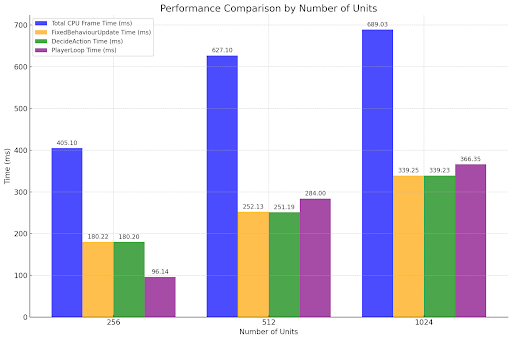
\includegraphics[width=0.5\textwidth]{figure 10.png} 
    \caption{CPU Performance For Hidden Units}
    \label{fig:CPU Performance For Hidden Units}
\end{figure}

Finally if we look at the memory usage of all at Figure~\ref{fig:Total Commited Memory By Hidden Units}. We can see that there is no significant relation between the number of hidden units and total committed memory.

\begin{figure}[htbp]
    \centering
    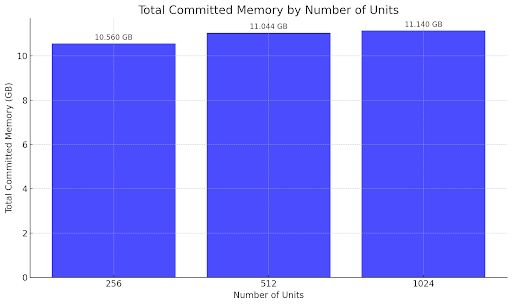
\includegraphics[width=0.5\textwidth]{figure 11.png} 
    \caption{Total Commited Memory By Hidden Units}
    \label{fig:Total Commited Memory By Hidden Units}
\end{figure}


% Conclusion
\section{Conclusion}
% Bibliography
\bibliographystyle{plain}
\bibliography{selectionsortBib}

\end{document}
